\chapter{Dziedzina problemu}

\begin{wrapfigure}{R}{3in}
%%%%%%%%%%%%%%%%%%%%%%%%%%%%%%%%%%%%%%%%%%%%%%%%%%%%%%%%%%%%%%%%%%%%%%%%%%%%%%%%%%%%%%%
%%% You will need to add \usepackage{wrapfig} to your preamble to use textwrapping %%%
%%%%%%%%%%%%%%%%%%%%%%%%%%%%%%%%%%%%%%%%%%%%%%%%%%%%%%%%%%%%%%%%%%%%%%%%%%%%%%%%%%%%%%%
 \centering
 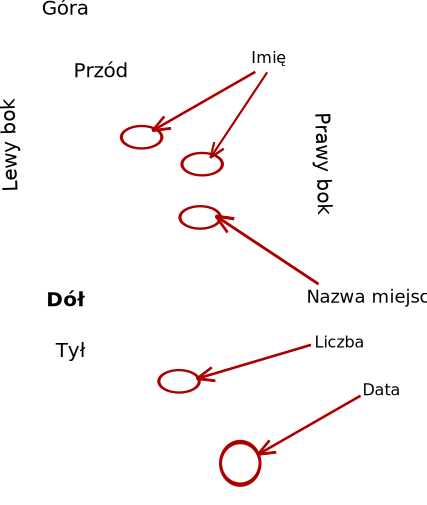
\includegraphics[width=150px]{../diagramy/tabliczka.pdf}
 % tabliczka.pdf: 342x405 pixel, 72dpi, 12.06x14.29 cm, bb=0 0 342 405
 \caption{Gliniana tabliczka - struktura}
\end{wrapfigure}


% \begin{figure}[h]
%  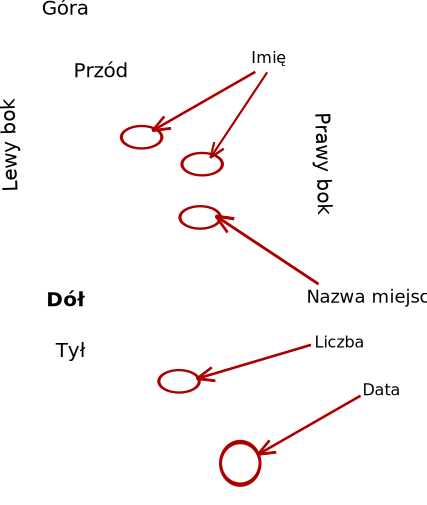
\includegraphics[width=150px]{../diagramy/tabliczka.pdf}
%  % tabliczka.pdf: 342x405 pixel, 72dpi, 12.06x14.29 cm, bb=0 0 342 405
%  \caption{Gliniana tabliczka - struktura}
% \end{figure}

\begin{figure}
 \centering
 
\includegraphics[width=400px]{../diagramy/Model-dziedziny.pdf}
 % Model-dziedziny.png: 650x345 pixel, 72dpi, 22.93x12.17 cm, bb=0 0 650 345
 \caption{Co powinna zawierać tabliczka w formie elektronicznej}
\end{figure}
~ 

Głównym pojęciem dziedziny jest tabliczka rozumiana dwojako - jako fizyczna tabliczka gliniana lub jako tabliczka w formie cyfrowej. 
Jej najważniejszym elementem jest treść zapisana klinami (w tabliczce glinanej) lub odczytami (w tabliczce elektronicznej), która 
może zawierać elementy znaczące, takie jak imię 
osoby, imię bóstwa, liczba, jednostka (np. przy opisywaniu wypłat), miejsce, data. Część tych elementów można przetłumaczyć na 
współczesny język (np. jednostki przeliczyć na SI, datę opisową na datę liczbową BC). 
Ponadto gliniane tabliczki są zapisywane z różnych stron 
(od góry, z przodu, z tyłu itp), mogą też zawierać pieczęcie - co znajduje odzwierciedlenie w treści tabliczki elektronicznej. 

Niestety odczyty zawarte w cyfrowym zapisie tabliczki są jednym z wariantów tłumaczenia z klinów. 
Ponieważ cyfrowej wersji nie ma klinów, możliwe są pomyłki w tłumaczeniach, które ciężko zweryfikować.
Choć są one dosyć mało prawdopodobne, sumerolodzy chcieliby mieć możliwość wyszukiwania po alternatywnych tłumaczeniach aby się 
od nich uniezależnić.

% Są też uszkodzone fragmenty, które zostały cyfrowo zapisane w najróżniejszej formie.

Poza treścią tabliczki cyfrowa wersja zawiera także metadane informujące m. in. o jej miejscu znalezienia, czasie powstania, 
 kolekcji do której obecnie należy, publikacji, w której się pojawiła. 
Są one istotne, gdyż często pozwalają na określenie o czym jest tabliczka bez wczytywania się w jej treść. 
Jednym z atrybutów, który w znacznym stopniu pomaga zidentyfikować tabliczkę jest publikacja.



%TODO:spytać
% Sumerolodzy potrafią określić w przybliżeniu treść tabliczki na podstawie publikacji.
%TODO:ciągłość

Sumerolodzy oczekują możliwości wyszukiwania po metadanych, po treści tabliczki (odczyty) 
i po alternatywnych tłumaczeniach (po klinach).  %TODO: po klinach??
Dodatkowym plusem byłoby wyszukiwanie po tagach (ludziach, jednostkach, datach itp)
W pierwszej wersji języka implementujemy tylko wyszukiwanie po odczytach i metadanych.